% !TEX root =  master.tex
\chapter{Marketing-Mix, Kommunikationspolitik und Werbung}
\section{Marketing-Mix}
Der Marketingmix besteht aus der Produktpolitik, Kontrahierungspolitik, Kommunikationspolitik und der Distributionspolitik.

Die Produktpolitik beinhaltet den Kern des Produktes, sowie die Verpackung und die Markierungen. Die Produktpolitik steht meist an erster Stelle, denn ohne Produkt bzw. Dienstleistung  ist  jedes  Marketing  in  der  Praxis  sinnlos. 

Die Kontrahierungspolitik auch Preispolitik genannt, beinhaltet die Methode zur Preisbestimmung, diese können zum Beispiel Skimming (Abschöpfungsstrategie), Penetration und Zahlungsbedingungen sein.

Die Kommunikationspolitik ist die Marketingkommunikation, unter der man den Einsatz von Instrumenten des Marketings versteht, die das Unternehmen zur Übermittlung seiner auf den Absatzmarkt gerichteten Informationen einsetzt. Die kann die klassische Werbung, Sales Promotions oder PR-Aktionen sein.

Zuletzt kommt im 4P-Marketing-Mix die Distributionspolitik. Diese ist die Pipeline des Marketings und man kennt sie  unter dem Vertrieb des Marketings. Sie vereint die drei Teilbereiche Vertriebswege, Vertriebsorgane und Vertriebssysteme.
\begin{figure}[H]
	\centering
	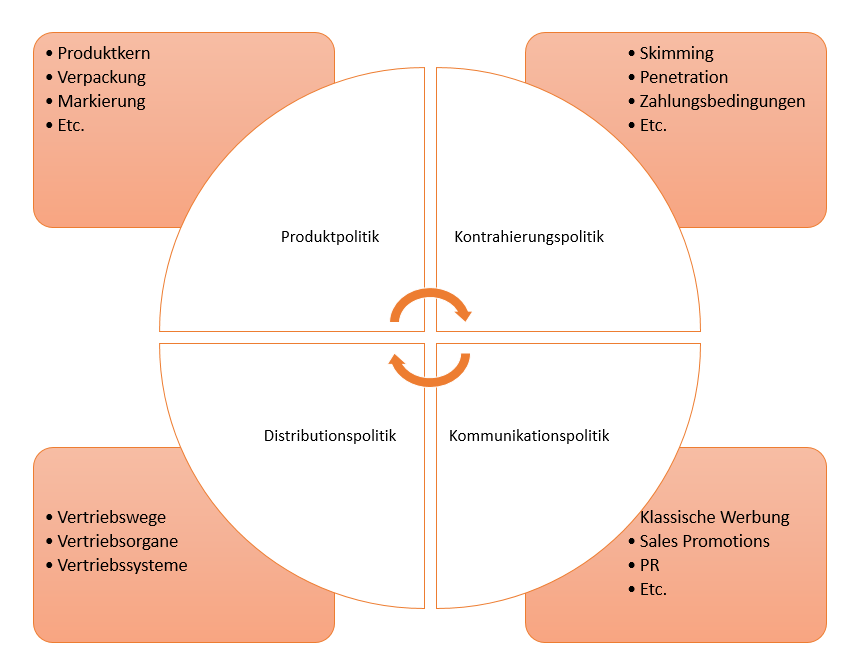
\includegraphics[width=1.0\linewidth]{img/MarketingMix}
	\caption[Marketing-Mix]{Marketing-Mix: Produkt-, Kontrahierungs-, Kommunikations- und Distributionspolitik}
	\label{fig:marketingmix}
\end{figure}


\autocite[Vgl.][]{MarketingMB}
\section{Kommunikationspolitik}
Die Kommunikationspolitik beinhaltet verschiedene Arten der Kommunikation. Es gibt sieben verschiedene, die unterschiedlich auf die Absatzförderung abzielen. 

Die \textbf{klassische Werbung} ist sehr unpersönliche Art der Kommunikation. Durch diese Art werden die Zielgruppen mit Absicht und ohne Zwang durch den Einsatz von gewissen Werbemitteln beeinflusst. Das Ziel ist die marktökonimsche Optimierung. Das bedeutet das Steigern von Umsatz, Absatz, Marktanteile, Deckungsbeiträge und dem ROI. Zudem soll der Bekanntheitsgrad gesteigert werden und ein Image aufgebaut werden. Diese zählen zu den marktpsychologischen Impulsen.
Um dies zu erreichen werden gewisse Mittel verwendet. Diese Mittel sind das Werbeobjekt, Werbesubjekt, Werbetreibender, Werbebotschaft, Werbemittel und der Werbeträger.

Das Werbeobjekt sind die Produkte oder Dienstleistungen, für die geworben werden. 

Das Werbesubjekt ist die Zielgruppe oder Zielperson, die durch die Werbung angesprochen werden soll. Es können auch bestimmte Unternehmen angeworben werden.

Der Werbetreibende ist eine Person oder ein Unternehmen, die den Auftrag der Werbung ausführen. Sie werben um das Werbesubjekt mit dem Werbeobjekt.

Die Werbebotschaft sind Informationen, die dem Werbesubjekt in verschiedenen Formen, wie Wort, Bild und Ton vermittelt werden sollen.

Das Werbemittel ist eine gestaltende (objektivierte) Form der Werbebotschaft. Das können Anzeigen in Zeitschriften, Werbespots im Fernsehen oder im Radio sein.

Der Werbeträger ist das Mittel, mit dem die Werbung dargestellt werden soll oder wo sie publiziert werden soll. Es ist der Träger des Werbemittels zum Werbeobjekt. Das sind zum Beispiel Zeitungen, Fernsehsender, Zeitschriften und viele weitere.

Das bekannteste Modell der Literatur für die Wirkung von Werbung ist das AIDA-Modell von Lewis. Es geht darum, dass die Werbung Aufmerksamkeit erzeugt (Attention). Die Zielgruppen sollen die Werbung wahrnehmen. Es geht darum so auffällig wie möglich zu Werben und alle Reize der Menschen auf sich zu ziehen, damit eine Fokus auf das Werbeobjekt entsteht. Daraufhin soll die Zielgruppe sich eine Meinung zu dem Produkt bilden. Sie soll die Meinung einnehmen, dass das Objekt einen Mehrwert für sie liefert und es dringend benötigt wird (Interest). Eine weitere Steigerung der Interesse und Stimulation soll ein Bedürfnis nach dem Objekt fördern, damit die Menschen unzufrieden sind, wenn sie das Objekt nicht besitzen (Desire). Das Verlangen wird verstärkt. Um das Verlangen zu stoppen, soll die Zielgruppe das Objekt kaufen und ihre verbundene Unzufriedenheit beseitigen (Action).

Die \textbf{Verkaufsförderung} oder auch \textbf{Sales Promotion} genannt, spiegelt die Hauptcharakteristik der Verkaufsförderung wieder und unterscheidet dadurch zu klassischen Werbung. Bei der Verkaufsförderung findet die Förderung immer am Verkaufsort statt. Damit sind Einzelhandelsfilialen gemeint. Da es viele verschiedene Zielgruppen gibt, wird die Verkaufsförderung in drei verschieden Arten unterteilt. Es gibt die Verbraucherpromotions, Verkäuferpromotions und die Handelspromotions.

\enquote{Bei der Option der Verbraucherpromotions steht der Endverbraucher im Zentrum  der  Verkaufsförderung-Aktivitäten.  Man  beabsichtigt  dabei konkret, die Quote der ungeplanten  Einkäufe  („Spontankäufe“)  durch  spezielle  Impulse  zu  maximieren.  Besonders  bewährt  haben  sich  dabei  Verkostungen,  Samples,  Displays für  Zweitplatzierungen,  Sonderpreisaktionen  oder  auch  Deckenwipper  und Regalstopper. } \autocite[Vgl.][]{MarketingMB}

\enquote{Bei der Verkäuferpromotions sollen die Verkäufer des Einzelhandels durch die Verkaufsförderung- Maßnahmen des Herstellers dazu bewegt werden, die Produkte dieses Herstellers  im  Kundenkontakt  besonders  zu  empfehlen.  Beliebte  Instrumente sind dabei Verkaufswettbewerbe, Verkaufstrainings, Salesfolder und andere. } \autocite[Vgl.][]{MarketingMB}

\enquote{Die handelsorientierte Verkaufsförderung erfolgt in der Regel ohne Herstellerbeteiligung. Der Einzelhändler versucht mit dem Einsatz dieses  Instrumentes  einen  Imagegewinn  und  eine  höhere  Ladentreue  beim Endverbraucher  zu  generieren.  Dazu  gestaltet  er  beispielsweise  kundenfreundliche  Jahreszeiten-Events  (Beispiel:  „Der  Globus  Weihnachts-Basar“) oder er setzt Kundenkarten und Treueaktionen ein.} \autocite[Vgl.][]{MarketingMB}

\textbf{Product Placement} ist in Deutschland als \textbf{Schleichwerbung} bekannt und weitesgehend verboten. Die werbewirksame Integration von Produkten und/oder  Dienstleistungen  in  Medienprogramme werden unter Product Placement verstanden. Diese finden im Kino, auf DVDs oder im Fernsehprogramm statt. Ganz bekannt sind heutzutage auch You-Tube Videos oder Beiträge bei Instagram. Das Ziel ist es die Marktstellung und den Erfolg dazu zu verbessern/steigern. Product Placement kann in ganz vielen verschiedenen Formen auftreten, diese sind abhängig von dem Klassifikationsmerkmal.

\begin{figure}[H]
	\centering
	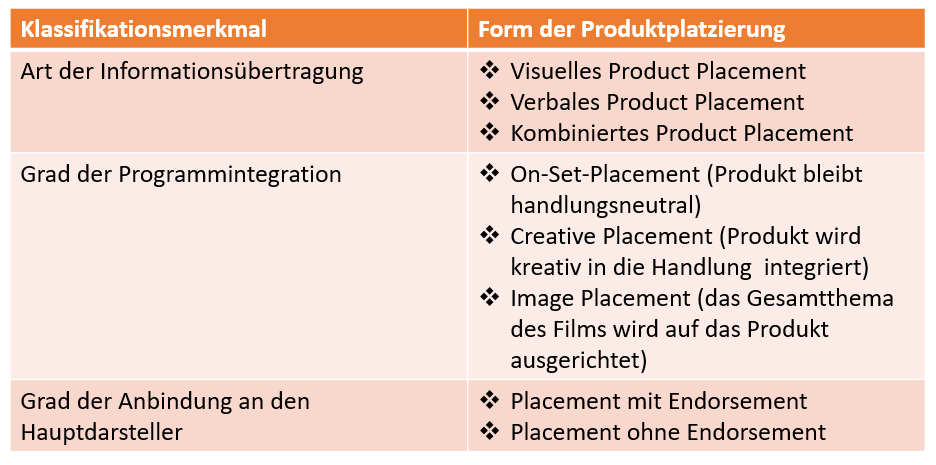
\includegraphics[width=1.0\linewidth]{img/ProductPlacement}
	\caption[Product Placement Formen]{Product Placement Formen}
	\label{fig:productplacement}
\end{figure}


Unter \textbf{Sponsoring} versteht man, dass ein Sponsor einem Gesponsorten Geld oder Sachmittel zu Verfügung stellt und eine Gegenleistung erhält. Diese Gegenleistung hat das Ziel die Marketing-Ziele des Sponsors zu erreichen. Es gibt heutzutage viele verschiedene Arten des Sponsoring:

\begin{enumerate}
	\item Sport-Sponsoring
	\item Kultur-Sponsoring
	\item Sozial-Sponsoring
	\item Öko-Sponsoring
	\item Programm-Sponsoring
\end{enumerate}

Die Kommunikationsform \textbf{Public Relations} \enquote{bezeichnet die planmäßige, systematische und wirtschaftlich sinnvolle  Gestaltung  der  Beziehungen  zwischen  einer  Unternehmung  und  einer  nach Gruppen gegliederten Öffentlichkeit mit dem Ziel, bei diesen Teilöffentlichkeiten Vertrauen und Verständnis aufzubauen.}.
Die PR-Arbeit wird in fünf Formen und acht Funktionen eingeteilt.

Die Formen der PR-Arbeit sind:

\begin{enumerate}
	\item Pressearbeit
	\item Maßnahmen  des  persönlichen  Dialogs
	\item Ausgewählte  Aktivitäten  für  Zielgruppen
	\item PR-bezogene  Mediawerbung
	\item Unternehmensinterne Maßnahmen
\end{enumerate}

Die Funktionen der PR-Arbeit sind:

\begin{enumerate}
	\item Informationsfunktion 
	\item Kontaktfunktion  
	\item Führungsfunktion  
	\item Imagefunktion  
	\item Harmonisierungsfunktion 
	\item Absatzförderungsfunktion  
	\item Stabilisierungsfunktion  
	\item Kontinuitätsfunktion  
\end{enumerate}

Mit der Kommunikationsform Public Relations gehen auch Corporate Identity Maßnahmen einher. Diese sind extern und intern, denn \enquote{hochmotivierte  Mitarbeiter,  die  sich  maximal  mit  ihrem  Unternehmen  und  seinen Angeboten  identifizieren,  sind  auch  in  der  Lage,  bei  den  relevanten  Teilöffentlichkeiten  Vertrauen  und  Verständnis  aufzubauen.  Gegenüber  den  Mitarbeitern  zeigt sich  die  praktizierte  Corporate Identity  beispielsweise  im  Führungsstil,  in  der  Motivation  und  Förderung der Mitarbeiter sowie in der Entgeltpolitik.}.

Das \textbf{Direktmarketing} zielt wie die anderen nicht auf eine gewisse Masse ab, sondern wird direkt an eine Person adressiert. Es lässt sich in Kommunikation und Distribution unterteilen. Die Kommunikation beinhaltet die Direkt-Werbung und das Direct-Response-Marketing, während die Distribution den direkten Vertrieb und den Mailorder Versandhandel beinhaltet. 

Die direkte Werbung ist eine gezielte Einzelansprache. Einzelne Informationen, wie Vorname, Name, Adresse, Telefon, Familienstand und Geburtsdatum sind bekannt. Das Kaufverhalten wird zudem dokumentiert und dementsprechend ausgewertet. Diese Mittel werden heutzutage immer mehr eingeschränkt, da immer mehr Daten von Personen gesammelt und verarbeitet werden.

Das Direct-Response-Marketing dagegen ist ein Prozess aus mehreren Stufen.

\begin{enumerate}
	\item \enquote{Der anonyme Adressat kommt in Kontakt mit unadressierter Massenwerbung (Plakat, Postwurfsendung, Flyer etc.). Bei dieser Massenwerbung ist die Möglichkeit der Kontaktaufnahme via Telefonnummer oder per Post-Coupon explizit inkludiert.}
	\item \enquote{Bei der anschließenden Kontaktaufnahme gibt der Adressat an, dass er Interesse an dem beworbenen Produkt hat und hinterlässt seinen Namen, seine Adresse, seine Geburtsdaten, seinen Familienstand etc. }  
	\item \enquote{In der dritten und vorerst abschließenden Stufe des  Direct-Response-Marketings erhält der Adressat dann Direktwerbung}  
\end{enumerate}


Der Direkt-Vertrieb ist dagegen bekannt dafür, dass Handelsstufen übersprungen werden und eine direkte Verbindung zwischen Hersteller und Endabnehmer hergestellt wird. Der Hersteller überspringt so den Einzelhandel und hat so die vollkommene Kontrolle über das Geschäft und kann direkt mit dem Kunden in Kontakt treten und somit den gesamten Gewinn einkassieren, ohne, dass er mit dem Einzelhändler teilen muss.
Mögliche Arten des direkten Vertriebs sind zum Beispiel:

\begin{enumerate}
	\item Haustürgeschäfte 
	\item Party-Selling  
	\item Messen  und  Ausstellungen  
	\item Automatenverkauf  
	\item Factory  Outlet  Center 
	\item Eigene Shops des Herstellers
	\item Regionale Hofläden und Marktstände in der landwirtschaftlichen Produktion 
\end{enumerate}
 
Der Mailorder Versandhandel ist eine ältere Version und ist kurz vor dem Aussterben. Der Kunde hat in Verkaufs-Katalogen seine Produkte gesichtet und schriftlich per Post oder per Telefon die Ware beordert. Die Ware wurde daraufhin per Post verschickt.

Die letzte Form der Kommunikation ist das \textbf{Online-Marketing}. Es gehört nicht direkt zum Direktmarketing, ist jedoch eine Subgruppe davon und hat in den letzten Jahren enorm zugenommen. Es lässt sich, wie das Direktmarketing, in Kommunikation und Distribution unterteilen. Die Kommunikation beinhaltet hier jedoch E-Mail, Newsletter und Banner, Popups, Spam und vieles mehr, während die Distribution den E-Commerce  und E-Business beinhaltet. 

\enquote{Innerhalb der Kommunikationspolitik gibt es, analog zum Direktmarketing, zum einem die  Option  der  adressierten  und  personalisierten  Einzelansprache.  Die  häufigsten Werbemittel sind hierbei E-Mail und Newsletter. Zum anderen kann ein mehrstufiger, im  ersten  Schritt  anonymer,  Dialog  zur  Generierung von  persönlichen  Daten  (sog. „Leads“)  eingesetzt  werden.  Die  wichtigsten  Werkzeuge  dazu  sind  Banner,  Popups und Spam-Mails. }. \autocite[Vgl.][]{MarketingMB}

Bei der Distribution unterscheidet man zwischen E-Commerce und E-Business. Als E-Commerce bezeichnet man den Handel von Produkten und Dienstleistungen über das Internet, während das E-Business das Geschäft im Internet ist, über das der Handel abgewickelt wird.
\autocite[Vgl.][]{MarketingMB}

\section{Werbung}
\subsection{Was ist Werbung?}
Werbung ist laut dem Duden ein Synonym für die Begriffe \enquote{Absatzförderung, Hype, Medienpräsenz oder auch für Öffentlichkeitsarbeit}. \autocite[Vgl.][]{DudenMB} Es ist ein Teil des Marketing-Mixes und wird durch eine Form der Kommunikation dargestellt. Durch Werbung können spezifische Gruppen angesprochen werden, in dem durch bestimmte Kommunikationsmittel verhaltensrelevante Einstellungen der Zielgruppen beeinflusst werden. Werbung ist das bekannteste und ein sehr effektives Marketing-Mittel und begegnet einem jeden Tag. \autocite[Vgl.][]{GablerMB} Es gibt zahlreiche Werbesprüche, die im Kopf bleiben. Dies bedeutet, dass das Ziel die Menschen erreicht zu haben, erfolgreich war. Man kennt es noch von seinen Eltern, die bekannte Werbesprüche aus ihrer Kindheit aufsagen können oder auch unserer Generation, die mit Sprüchen, wie \enquote{Haribo macht Kinder froh und Erwachsene ebenso} \autocite[Vgl.][]{HariboMB} oder \enquote{Waschmaschinen leben länger mit Calgon} \autocite[Vgl.][]{CalgonMB} aufgewachsen sind. 

\subsection{Wie kann Werbung eingesetzt werden?}
Für die MOBTS an der DHBW in Mannheim kann man vielseitige Werbemaßnahmen treffen. Die DHBW Mannheim verfügt über eine Internetpräsenz, die genutzt werden kann, die Studenten und DHBW-Interessierte anzulocken. Zusätzlich gibt es verschiedene Studenteneinrichtungen der DHBW, die im Internet auf verschiedenen Social Media Plattformen vertreten sind. Es sollten Maßnahmen ergriffen werden, dass diese Plattformen genutzt werden und dort Werbevideos oder auch einfache Beiträge geteilt werden, damit die MOBTS an der DHBW in Mannheim eine größere Zielgruppe erreicht. Zusätzlich können Artikel in Zeitschriften in Mannheim und Umgebung veröffentlicht werden, die nicht nur die jüngeren Generationen im Internet erreichen, sondern auch andere Generationen, die nichts mit der Social Media Welt zu tun haben und gegebenenfalls auch nichts mit der DHBW oder der MOBTS. Da die DHBW ein Partner von vielen Unternehmen, sei es ein Kleinunternehmen oder ein Big Player, ist, sollten hier Ansprechpersonen gefunden werden, damit Werbung in den Unternehmen gemacht werden kann. Es gibt zahlreiche Möglichkeiten, die genutzt werden sollten. Alleine eine Anzeige auf der Internetseite der MOBTS oder der DHBW Mannheim reicht nicht, dmait ein größeres Publikum angelockt wird. Das Werbevideo ist ein erster Schritt und zeigt eine Initiative das Marketing voranzutreiben. Die erstellten Flyer können zahlreich verteilt werden und auch digital abgebildet werden, damit eine geeignete Marketingstrategie stattfinden kann. 
\subsection{Welchen Nutzen kann aus Werbung gezogen werden?}
Der Nutzen der Werbemaßnahmen kann einen positiven Erfolg auf das Event und auf die DHBW in Mannheim haben. Die DHBW Mannheim erreicht somit eine größere Zielgruppe und kann so Studenten für die Zukunft für sich gewinnen. Denn so zeigt sie, dass die DHBW eine gewisse Bandbreite hat, die angehende Studenten gefallen könnte. Nicht nur können so neue Studenten angeworben werden, sondern auch gegebenenfalls neue Dozenten, die an solch einer Einrichtung, die internationale Tagungen austrägt, dozieren möchten. Durch neue Dozenten ist es auch möglich neue Praxispartner zu gewinnen, die das Konzept der DHBW dadurch besser kennenlernen und dort ihre neuen Studenten unterbringen möchte. 

Generell ist zu sehen, dass durch die heutigen Generationen und der Corona-Pandemie eine Internetpräsenz sehr wichtig und wertvoll ist. Selbst durch kleinere Maßnahmen, wie ein einziger Beitrag in Social Media, kann ein gewisser Hype entstehen und viele Leute erreicht werden. Durch einen gut durchstrukturierten und auffälligen Beitrag kann die Aufmerksamkeit vieler auf sich gezogen werden, die über kurz oder lang auf der Internetseite der MOBTS oder DHBW Mannheim landen. Dadurch ist ein erstes Interesse geweckt und zusätzliche Besucher und Interessenten können so entstehen.

Die DHBW in Mannheim sollte dadurch all ihre Studenten dazu einladen an der MOBTS teilzunehmen und mit gewissen Speakern werben, die für einige sehr von Interesse sein könnten und somit eine größere Präsenz und Aufmerksamkeit erreichen.

